\documentclass{beamer}
\usepackage[english,russian]{babel}
\usepackage{amsmath}
\usepackage{amsfonts}
\usepackage[utf8]{inputenc}
% Стиль презентации
\usetheme{boxes}
\begin{document}
\title{Сегментация  изображений}  
\author{Костенко Дмитрий}

\date{Москва, 2013} 
% Создание заглавной страницы
\frame{\titlepage}




\begin{frame}{Формальное определение}
\frametitle{Определение}
Сегментация — это процесс разделения цифрового изображения на несколько сегментов (множеств пикселей).
\end{frame}


\begin{frame}{Пример}
\frametitle{Проще говоря}
Это процесс, в результате которого мы определим какие пиксели из данного множества относятся к красной машине, а какие к синей. 

 \begin{center}
  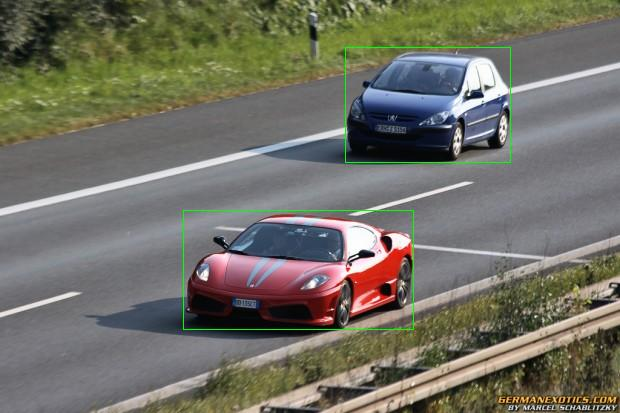
\includegraphics[width= 0.8\linewidth]{images/cars.jpg}  
 \end{center}
 
\end{frame}




\begin{frame}{Трудности}
\frametitle{Трудности}
Сложный фон
 \begin{center}
  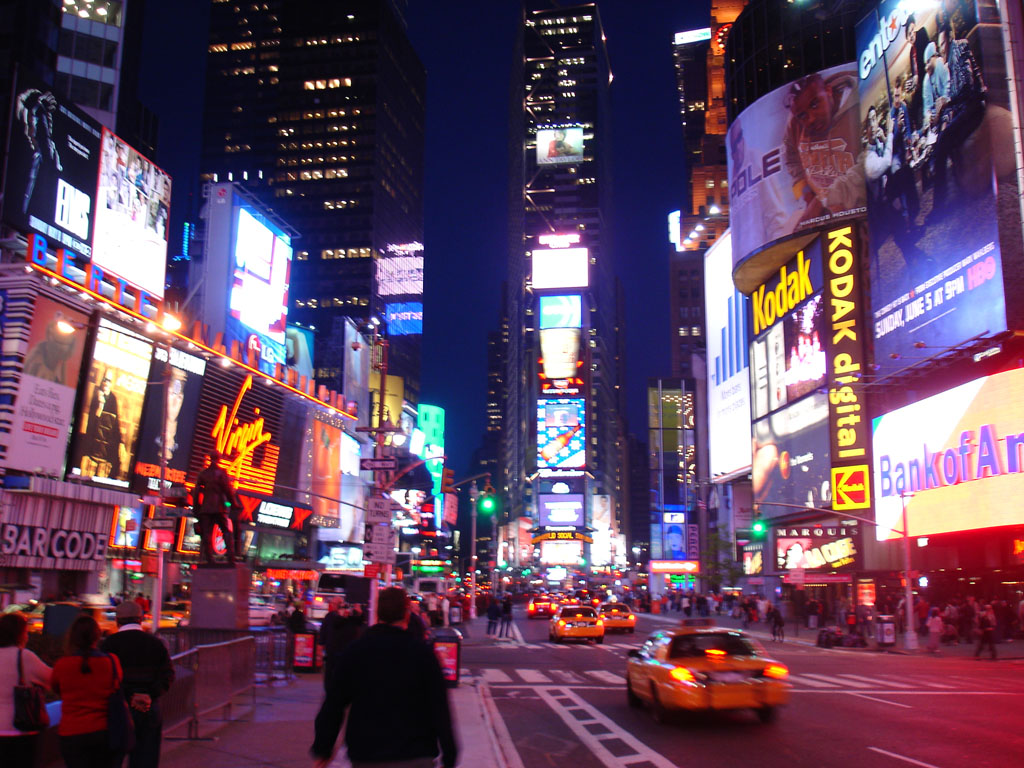
\includegraphics[width= 0.8\linewidth]{images/complex_background.jpg}  
 \end{center}
\end{frame}



\begin{frame}{Трудности}
\frametitle{Трудности}
Перекрытие объектов
 \begin{center}
  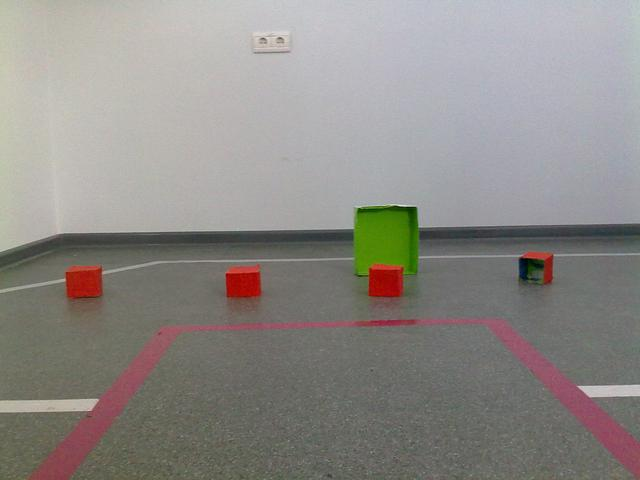
\includegraphics[width= 0.8\linewidth]{images/overlap.jpg}  
 \end{center}
\end{frame}


\begin{frame}{Типы сегментаций}
\frametitle{Типы сегментаций}
 \begin{center}
  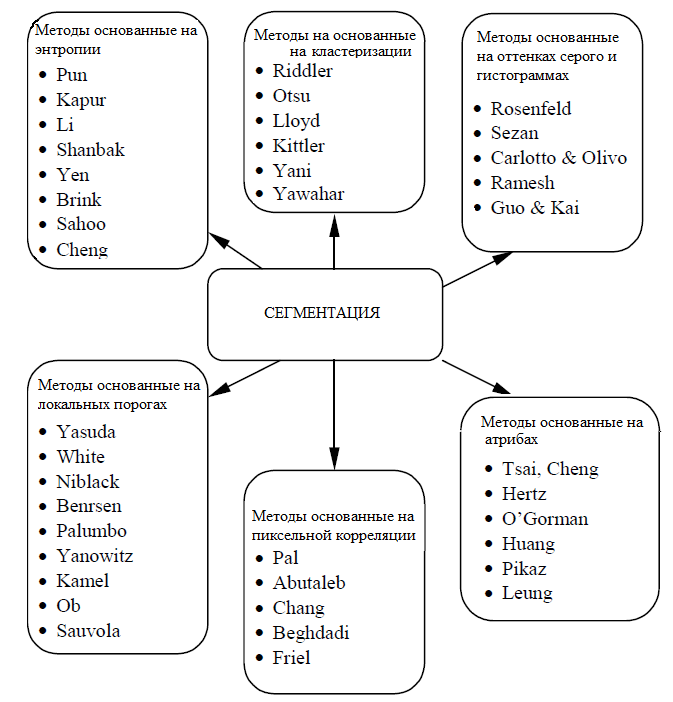
\includegraphics[height= 0.8\linewidth]{images/types.png}  
 \end{center}
\end{frame}


\begin{frame}{Бинаризация}
\frametitle{Бинаризация}
 \begin{center}
  Бинаризация с нижним (или верхним) порогом является наиболее простой операцией, в которой используется только одно значение порога: 
  
  \[
f'(m,n) = \left\{ 
  \begin{array}{l l}
    0 & \quad \text{если $f(m,n)$ > t}\\
    1 & \quad \text{если $f(m,n)$ $\leqslant$  t}
  \end{array} \right.
  \]
  
 \end{center}
\end{frame}


\begin{frame}{Бинаризация}
\frametitle{Бинаризация}
 \begin{center}
	\begin{itemize}
		\item Бинаризации с нижним порогом
 		\item Бинаризации с верхним порогом
  		\item Бинаризация с двойным ограничением
  		\item Неполная пороговая обработка
  		\item Многоуровневое пороговое преобразование
	\end{itemize}
 \end{center}
\end{frame}


\begin{frame}{Метод Оцу}
\frametitle{Метод Оцу}
  Метод использует гистограмму распределения значений яркости пикселей растрового изображения. Строится гистограмма по значениям 		  $p_{i} = n_{i} / N$
  
  где 
  
  N – это общее кол-во пикселей на изображении, 
  
  $n_{i}$ – это кол-во пикселей с уровнем яркости i. 
\end{frame}




\begin{frame}{Метод Оцу}
\frametitle{Метод Оцу}
 \begin{center}
  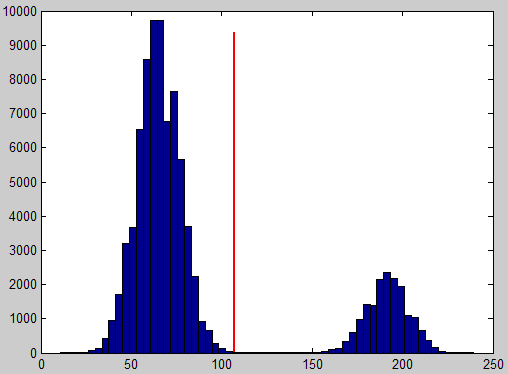
\includegraphics[width= 0.8\linewidth]{images/gist.png}  
 \end{center}
\end{frame}




\begin{frame}{Метод Оцу}
\frametitle{Метод Оцу}
  Диапазон яркостей делится на два класса с помощью порогового значения уровня яркости k.
  
  k — целое значение от 0 до L. 
  
  Каждому классу соответствуют относительные частоты $\omega_{1}$ $\omega_{2}$:
  
  $$ \omega_{0}(k) = \sum_{i=1}^{k} p_{i} $$
  $$ \sum_{i=k+1}^{L} p_{i} = 1 - \omega _{0} (k) $$
  
  $$\mu _{0}(k) = \sum_{i=1}^{k} \frac{ip_{i}}{\omega _{0}} $$
  $$\mu _{1}(k) = \sum_{i=k+1}^{L} \frac{ip_{i}}{\omega _{1}} $$
\end{frame}





\begin{frame}{Метод Оцу}
\frametitle{Метод Оцу}
Далее вычисляется максимальное значение оценки качества разделения изображения на две части:
$$\sigma  _{\omega}^{2} (t)  = \omega _{1}(t) \sigma _{1}^{2} + \omega _{2}(t) \sigma _{2}^{2}$$

где $\omega _{i}$ — это вероятности двух классов, разделенных порогом t
$\sigma _{2}^{i}$ - дисперсия этих классов.
\end{frame}






\begin{frame}{Метод Оцу}
\frametitle{Метод Оцу}
	\begin{itemize}
		\item Вычислить гистограмму и вероятность для каждого уровня интенсивности.
 		\item Вычислить начальные значения для $\omega _{i} (0)$ и $\mu  _{i} (0)$.
  		\item Для каждого значения порога от t = 1 .. до максимальной интенсивности:
  		\begin{itemize}
  			\item Обновляем $\omega _{i}$ и $\mu _{i}$ 
  			\item Вычисляем $\sigma _{b}^{2} (t)$
  			\item Если $\sigma _{b} (t)$ больше, чем имеющееся, то запоминаем $\sigma _{b}$ и значение порога t.
  		\end{itemize}
  		\item Искомый порог соответствует максимуму $\sigma _{b}^{2} (t)$
	\end{itemize}
\end{frame}


\begin{frame}{Пример использования}
\frametitle{Пример использования}
	Локализация штрих-кода на изображении
 \begin{center}
  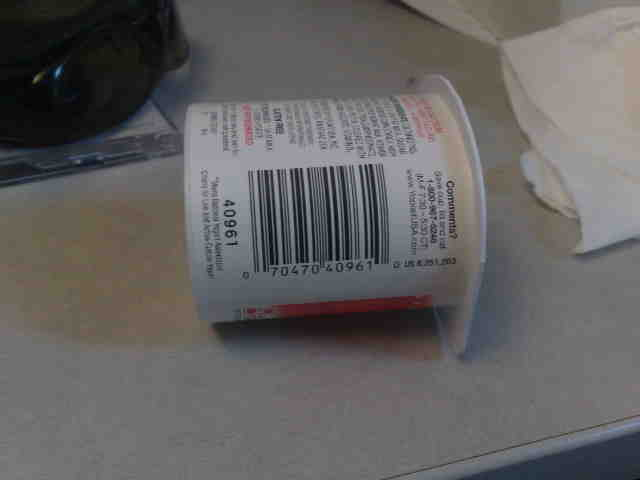
\includegraphics[width= 0.8\linewidth]{images/11.jpg}  
 \end{center}
\end{frame}

\begin{frame}{Пример использования}
\frametitle{Пример использования}
Взять изображение как разницу горизонтальной и вертикальной производной.

Далее применить усредняющий фильтр.
 \begin{center}
  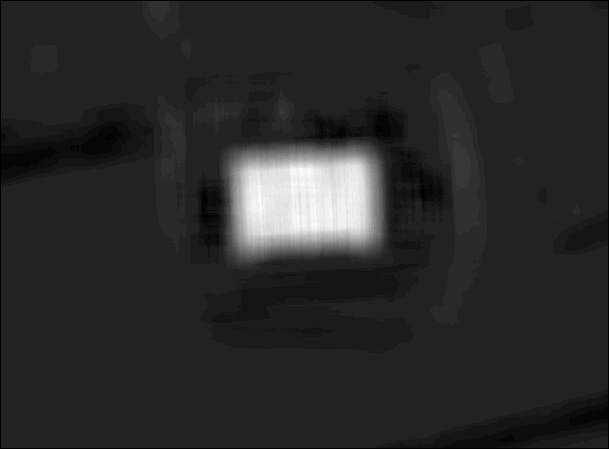
\includegraphics[width= 0.8\linewidth]{images/22.jpg}  
 \end{center}
\end{frame}

\begin{frame}{Пример использования}
\frametitle{Пример использования}
Результат метода Оцу
 \begin{center}
  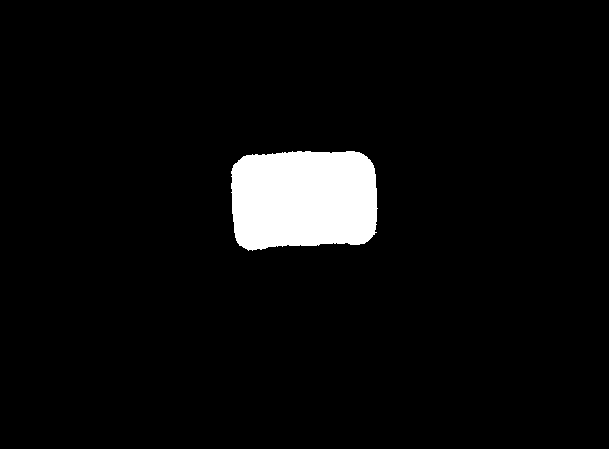
\includegraphics[width= 0.8\linewidth]{images/33.png}  
 \end{center}
\end{frame}


\begin{frame}{Достоинства}
\frametitle{Достоинства}
	\begin{itemize}
		\item Простота реализации.
 		\item Метод хорошо адаптируется к различного рода изображения, выбирая наиболее оптимальный порог.
  		\item Быстрое время выполнения. Требуется O(N) операций, где N — количество пикселей в изображении.
  		\item Метод не имеет никаких параметров, просто берете и применяете его. В MatLab это функция graythresh() без аргументов.
	\end{itemize}
\end{frame}

\begin{frame}{Недостатки}
\frametitle{Недостатки}
	\begin{itemize}
		\item Сама по себе пороговая бинаризация чувствительна к неравномерной яркости изображения.
	\end{itemize}
	
	Решением такой проблемы может быть введение локальных порогов, вместо одного глобального.
\end{frame}





\end{document}